% vim: set spell spelllang=en tw=100 et sw=4 sts=4 :

\documentclass[runningheads]{llncs}

\usepackage{tikz}
\usetikzlibrary{shapes, positioning, decorations.text}
\usepackage{cleveref}

\usepackage{listings}
\lstset{
basicstyle=\small\ttfamily,
mathescape,
escapeinside={(*}{*)},
numbers=none,
keywordstyle=\bfseries\color{blue},
keywords = {language, Essence, given, letting, find, such, that,
            bool, int, matrix, enum, variant, record, set, mset,
            sequence, function, relation, partition, 
            domain, total, surjective, be,
            forAll, exists, sum, injective, in, preImage, range,
            new, type, intersect, union, from,
            minimising, maximising, of, indexed, by, and,
            defined, maxSize, maxNumParts, size, regular, language, cheese
            }
showstringspaces=false,
tabsize=1,
breaklines=true,
breakatwhitespace=false,
}

\usepackage{showframe}

\title{Finding Subgraphs With Side Constraints}
\author{
    \"Ozg\"ur Akg\"un\inst{1} \and Jessica Enright\inst{2} \and Christopher
    Jefferson\inst{1} \and Ciaran McCreesh\inst{2} \and Patrick
    Prosser\inst{3} \and Steffen Zschaler\inst{4} \\
}
\authorrunning{\"O. Akgun et al.}
\institute{
    University of St Andrews, Scotland \and
    University of Glasgow, Scotland \\ \email{ciaran.mccreesh@glasgow.ac.uk} \and
    Algorithmicists Anonymous (Machrihanish), Scotland \and
    King's College London, England
}

\crefname{Figure}{Figure}{Figures}
\crefname{figure}{figure}{figures}

\begin{document}

\maketitle

\begin{abstract}
    The subgraph isomorphism problem is to find a small ``pattern'' graph inside a larger ``target''
    graph. There are excellent dedicated solvers for this problem, but they require substantial
    programming effort to handle complex side constraints; however, general purpose constraint
    solvers struggle on more difficult graph instances. We show how to combine the state of the art
    Glasgow Subgraph Solver with the Minion constraint programming solver to get a ``subgraphs modulo
    theories'' solver that is both performant and flexible. We also show how such an approach can be
    driven by the Essence high level modelling language. We give practical examples taken from
    ??applications.
\end{abstract}

\section{Introduction}

Finding or counting small ``pattern'' graphs inside larger ``target'' graphs is a widely applicable
hard problem, with applications including ??. This has led to the development of numerous dedicated
algorithms, with the Glasgow Subgraph Solver \cite{DBLP:conf/gg/McCreeshP020} being the current
state of the art \cite{DBLP:conf/gbrpr/Solnon19}. However, practitioners are often interested in
versions of the problem with additional restrictions, or side constraints. Some of these, such as
exact vertex labelling schemes, are trivial to include in a dedicated solver, but others currently
require either extensive programming or inefficient post-processing. This paper explores a different
approach: by allowing the Glasgow Subgraph Solver to use the Minion constraint programming (CP) solver
\cite{DBLP:conf/ecai/GentJM06} for side constraints, we achieve both the performance only a
dedicated solver can offer, with the flexibility of a full CP toolkit. This
hybrid modelling system can be driven by the Essence high level modelling language
\cite{DBLP:journals/constraints/FrischHJHM08}, making it accessible to non-specialists.

\subsection{Preliminaries}

We begin with a look at the subgraph isomorphism problem, from a high level constraint modelling
perspective.  The basic non-induced subgraph isomorphism problem is to find an injective mapping
from a pattern graph to a target graph, such that adjacent vertices in the pattern are mapped to
adjacent vertices in the target. Variations on the problem are common, and are often combined. For
example, in the induced version of the problem, non-edges must be mapped to non-edges; in the
directed version, the input graphs have directed edges whose orientations must be preserved by the
mapping; in the vertex labelled version, each vertex has a label, and the mapping must map vertices
to like-labelled vertices; and in the edge-labelled version, edges have labels which must be
preserved.  It is also common to want to count or enumerate all solutions, rather than deciding
whether at least one solution exists.  Subsets of these variations are all supported by many
dedicated subgraph isomorphism algorithms, including the Glasgow Subgraph Solver.

\begin{figure}[tb]
    \centering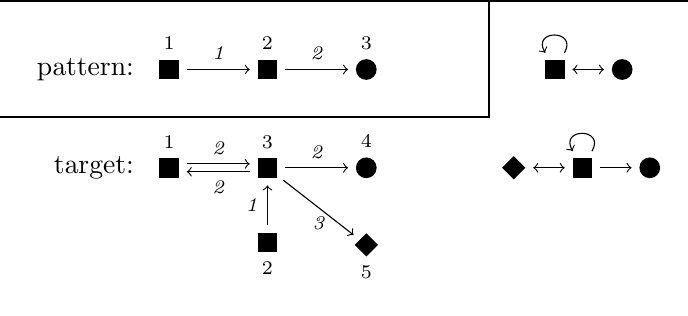
\begin{tikzpicture}
        \node [draw, fill] (P1) {}; \node [above=0cm of P1, font=\scriptsize] { 1 };
        \node [draw, fill, right=1cm of P1] (P2) {}; \node [above=0cm of P2, font=\scriptsize] { 2 };
        \node [draw, fill, circle, right=1cm of P2, inner sep=2.5pt] (P3) {}; \node [above=0cm of P3, font=\scriptsize] { 3 };
        \draw [->, shorten >=1mm, shorten <=1mm] (P1) -- (P2) node [midway, font=\scriptsize\itshape, above] { 1 };
        \draw [->, shorten >=1mm, shorten <=1mm] (P2) -- (P3) node [midway, font=\scriptsize\itshape, above] { 2 };
        \node [left=0.2cm of P1, anchor=east] { pattern: };

        \node [draw, fill, right=4.65cm of P1] (PT1) {};
        \node [draw, fill, circle, inner sep=2.5pt, right=0.6cm of PT1] (PT2) {};
        \draw [<->, shorten >=1mm, shorten <=1mm] (PT1) -- (PT2);
        \draw [->, shorten >=1mm, shorten <=1mm] (PT1) to [out=60, in=120, looseness=8] (PT1);

        \node [draw, fill, below=1cm of P1] (T1) {}; \node [above=0cm of T1, font=\scriptsize] { 1 };
        \node [draw, fill, right=1cm of T1] (T3) {}; \node [above=0cm of T3, font=\scriptsize] { 3 };
        \node [draw, fill, below=0.7cm of T3] (T2) {}; \node [below=0cm of T2, font=\scriptsize] { 2 };
        \node [draw, fill, circle, right=1cm of T3, inner sep=2.5pt] (T4) {}; \node [above=0cm of T4, font=\scriptsize] { 4 };
        \node [draw, fill, diamond, below=0.7cm of T4, inner sep=2pt] (T5) {}; \node [below=0cm of T5, font=\scriptsize] { 5 };
        \draw [->, shorten >=1mm, shorten <=1mm, transform canvas={yshift=0.5mm}] (T1) -- (T3) node [midway, font=\scriptsize\itshape, above] { 2 };
        \draw [<-, shorten >=1mm, shorten <=1mm, transform canvas={yshift=-0.5mm}] (T1) -- (T3) node [midway, font=\scriptsize\itshape, below] { 2 };
        \draw [->, shorten >=1mm, shorten <=1mm] (T2) -- (T3) node [midway, font=\scriptsize\itshape, left] { 1 };
        \draw [->, shorten >=1mm, shorten <=1mm] (T3) -- (T4) node [midway, font=\scriptsize\itshape, above] { 2 };
        \draw [->, shorten >=1mm, shorten <=1mm] (T3) -- (T5) node [midway, font=\scriptsize\itshape, below] { 3 };
        \node [left=0.2cm of T1, anchor=east] { target: };

        \node [draw, fill, right=5cm of T1] (TT1) {};
        \node [draw, fill, circle, inner sep=2.5pt, right=0.6cm of TT1] (TT2) {};
        \node [draw, fill, diamond, inner sep=2pt, left=0.6cm of TT1] (TT3) {};
        \draw [->, shorten >=1mm, shorten <=1mm] (TT1) -- (TT2);
        \draw [<->, shorten >=1mm, shorten <=1mm] (TT1) -- (TT3);
        \draw [->, shorten >=1mm, shorten <=1mm] (TT1) to [out=60, in=120, looseness=8] (TT1);
    \end{tikzpicture}
    \caption{A small pattern and a larger target graph used in examples throughout this paper. The
    plain text numbers are vertex names, and the shapes on vertices represent vertex labels. The
    graphs to the right are \emph{type graphs}, which are used in \cref{section:typegraphs}. The
    italic labels on edges are used for \emph{temporal graphs}, which are discussed in
    \cref{section:temporalgraphs}, and should otherwise be ignored.}
    \label{figure:littlegraphs}
\end{figure}

We can express these problems in the Essence high level modelling language, as follows. We assume
vertices take their labels from the set $L = \{ 1\ldots\ell \}$ for some given $\ell$, and edges
from $E = \{ 1\ldots{}e \}$ (and so $\ell$ and / or $e$ may be 1, for applications that do not use
labels on vertices and / or edges):
\begin{lstlisting}
given l, e : int
letting L be domain int(1..l)
letting E be domain int(1..e)
\end{lstlisting}
We take as input a pattern directed graph which has $p$ vertices (which we number from 1 to $p$, in
the set $P$), and a target directed graph which has $t$ vertices (numbered from 1 to $t$, the set
$T$). Each graph is represented as total function from vertices to vertex labels, and a
\emph{partial} function from pairs of (not necessarily distinct) vertices to edge labels:
\begin{lstlisting}
given p, t : int
letting P be domain int(1..p)
letting T be domain int(1..t)

given pat : function (P, P) --> E
given tgt : function (T, T) --> E
given plab : function (total) P --> L
given tlab : function (total) T --> L
\end{lstlisting}
Now we wish to find an injective mapping $f$:
\begin{lstlisting}
find f : function (total, injective) P --> T
\end{lstlisting}
that preserves vertex labels,
\begin{lstlisting}
such that forAll a : P .  plab(a) = tlab(f(a))
\end{lstlisting}
and directed edges, including their labels:
\begin{lstlisting}
such that forAll (a, b) in defined(pat) .
    pat((a, b)) = tgt((f(a), f(b)))
\end{lstlisting}

As a simple example, the following inputs show the problem instance represented in
\cref{figure:littlegraphs}. We have three different vertex labels (circle, square, and diamond), and
only a single edge type (which is directed; the numerical labels on edges are not used in this
section):
\begin{lstlisting}
letting l be 3
letting e be 1
\end{lstlisting}
We may now describe the pattern:
\begin{lstlisting}
letting p be 3
letting pat be function ((1, 2) --> 1, (2, 3) --> 1)
letting plab be function (1 --> 1, 2 --> 1, 3 --> 2)
\end{lstlisting}
and the target:
\begin{lstlisting}
letting t be 5
letting tgt be function ((1, 3) --> 1, (3, 1) --> 1,
  (2, 3) --> 1, (3, 4) --> 1, (3, 5) --> 1)
letting tlab be function (1 --> 1, 2 --> 1, 3 --> 1,
  4 --> 2, 5 --> 3)
\end{lstlisting}
And the Conjure tool tells us that there are exactly two solutions to the problem, as we would
expect:
\begin{lstlisting}
(1 --> 1, 2 --> 3, 3 --> 4)
(1 --> 2, 2 --> 3, 3 --> 4)
\end{lstlisting}
But what if our application requires induced isomorphisms? Then we can easily add the constraint
\begin{lstlisting}
such that forAll (a, b) : (P, P) .
    (f(a), f(b)) in defined(tgt) -> (a, b) in defined(pat)
\end{lstlisting}
And Conjure will now find us a single solution,
\begin{lstlisting}
(1 --> 2, 2 --> 3, 3 --> 4)
\end{lstlisting}
Supporting other problem variants and constraints is similarly straightforward, even if auxiliary
variables are required. For example, if instead we want to allow relabelling on vertex labels (which
is typically not supported by dedicated solvers), we could do the following:
\begin{lstlisting}
find r : function (total, injective) L --> L
such that forAll a : P .  r(plab(a)) = tlab(f(a))
\end{lstlisting}
and we would find two additional solutions,
\begin{lstlisting}
(1 --> 1, 2 --> 3, 3 --> 5)
(1 --> 2, 2 --> 3, 3 --> 5)
\end{lstlisting}
and if we removed the injective keyword for the relabelling, we would find a fifth mapping
\begin{lstlisting}
(1 --> 2, 2 --> 3, 3 --> 1)
\end{lstlisting}

\subsection{Experiments and Motivation}

\begin{figure}[tb]
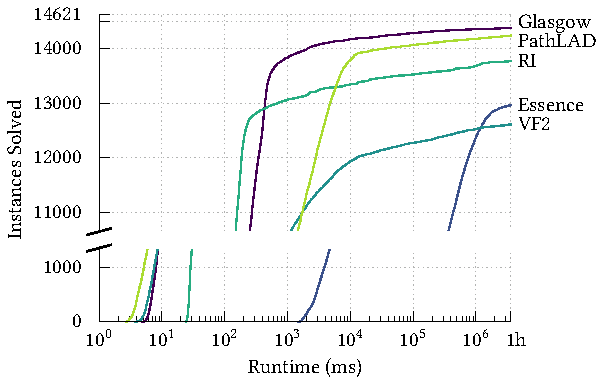
\includegraphics{gen-graph-glasgow-versus-minion-cumulative.pdf}\hfill\includegraphics*{gen-graph-glasgow-versus-minion-scatter.pdf}

    \caption{Left, the cumulative number of instances solved over time, for the non-induced decision
    problem with no side constraints. Right, comparing the high level approach with the Glasgow
    Subgraph Solver on an instance by instance basis; points on the outer axes represent
    timeouts.}\label{figure:solvers}
\end{figure}

Unfortunately, whilst elegant and flexible, the performance of this approach is rather terrible on
basic subgraph isomorphism instances.  We performed computational experiments on a cluster of
??fatanodes spec, using the ??14,621 unlabelled, undirected instances from Solnon's benchmark
suite\footnote{https://perso.liris.cnrs.fr/christine.solnon/SIP.html}. This benchmark suite was
originally designed for algorithm portfolios work \cite{DBLP:conf/lion/KotthoffMS16}, and brings
together several collections of application and randomly-generated instances with varying
difficulties and solution counts (including many unsatisfiable instances). Some of the instances
have up to ?? vertices and ?? edges in patterns and up to ?? vertices and ?? edges in
targets; these lead to rather large models, by constraint programming standards.

In \cref{figure:solvers} we plot the cumulative number of instances solved over time for
the non-induced decision problem, comparing the high level approach to the Glasgow Subgraph Solver
\cite{DBLP:conf/gg/McCreeshP020} and PathLAD \cite{DBLP:conf/lion/KotthoffMS16} (the two strongest
CP approaches), and to VF2 \cite{DBLP:journals/pami/CordellaFSV04} and RI
\cite{DBLP:journals/bmcbi/BonniciGPSF13} (simpler algorithms which perform well on easy instances).
The high level approach has very slow startup times (which is to be expected as it involves
launching a Java virtual machine), but much more worryingly, only just catches up with the worst
other solver in number of instances solved as the timeout approaches. Worse, as the scatter plot in
\cref{figure:solvers} shows, there are almost no instances where the high level approach
does better than the Glasgow Subgraph Solver. And, although not pictured, the situation for the
induced variant is even more pessimistic.

These first results motivate the remainder of this paper. We want to retain the convenience of the
high level modelling approach, and to be able to add arbitrary side constraints to suit different
applications, but we do not want to have to abandon the performance that dedicated solvers can get
on hard instances. In ??section we evaluate several ways of using a CP solver in
conjunction with the Glasgow Subgraph Solver, with a focus on low level implementation details. In
??section we then return to high level modelling, and look at the convenience it provides for
??temporal problems, ??relabelling and retyping, and ??optimisation problems.

\section{Hybrid Solving}

The Glasgow Subgraph Solver employs a CP approach to solve subgraph-finding problems, but using
special data structures and algorithms---for example, rather than representing the adjacency
constraint using a table, it uses bitset adjacency matrices. The solver also exploits various graph
invariants involving degrees and paths to further reduce the search space, and also has special
search order heuristics. From this paper's perspective, the most important design aspect is that
internally, the solver has a CP style variable for each vertex in the pattern graph, whose domains
range over the vertices of the target graph. The solver performs a backtracking search\footnote{The
solver also makes use of restarts and nogood recording, rather than just na\"\i{}ve backtracking,
but this does not hugely affect this paper.}
attempting to assign each variable a value from its domain, whilst respecting adjacency and
injectivity constraints. At each recursive call of search, the solver performs \emph{propagation} to
eliminate infeasible values from domains. If any domain becomes empty, the solver backtracks;
otherwise, it selects a variable, and tries assigning it each value from its domain in turn.

For now we will assume that there is some way of setting up the subgraph solver and a CP solver such
that they both have this same set of variables and values, and that there is some way of knowing how
to form a correspondence between their internal representations. We will allow the CP solver to have
additional variables that the subgraph solver does not know about (such as the second mapping used
in the relabelling example in the previous section), and we do not specifically require the CP
solver to be aware of all of the graph constraints.  This gives us several potential basic
approaches to handling side constraints:
\begin{itemize}
    \item We could use a CP solver as a \emph{solution checker}. Whenever the subgraph solver finds
        a solution, it will pass it to the CP solver, which will treat the solution as a set of
        equality constraints. The CP solver will then attempt to find a satisfying assignment. If
        the CP solver does not have any additional variables, this is equivalent to simply checking
        that the remaining constraints hold, but otherwise it can involve search. For a decision
        problem, the CP solver then communicates back to the subgraph solver either ``yes, this is a
        valid solution'', or ``no, reject this solution and keep going''. If we
        are solving a counting or enumeration problem, the CP solver must find \emph{all} solutions
        and communicate this back to the subgraph solver.
    \item We could additionally ask a CP solver at every stage of search to \emph{test} whether the
        state the subgraph solver is in is obviously infeasible. Whenever the subgraph solver has
        finished performing propagation, it can communicate the \emph{trail} (that is, its current
        sequence of guessed assignments) to the CP solver, which again treats these as additional
        equality constraints. The CP solver then performs its own propagation (but not search), and
        communicates back either a ``yes, keep going'' or a ``no, backtrack immediately''.
    \item Finally, after this testing, we could also ask the CP solver to communicate any deletions
        it infers back to the subgraph solver. In other words, the subgraph solver would use the CP
        solver as an additional propagator.
\end{itemize}
Unfortunately, each of these approaches has drawbacks. The solution we will settle upon is based
upon \emph{rollbacks}; we will describe this below, after presenting experiments that demonstrate
the difference between these approaches.

\subsection{Implementation}

?? How we do this: FIFOs, simple text based protocol. Both solvers are run and initialised. The
subgraph solver calls the CP solver as a propagator. The CP solver sets up the model, then clones it
and adds in new constraints for each query.

\subsection{Experiments}

\begin{figure}[p]
    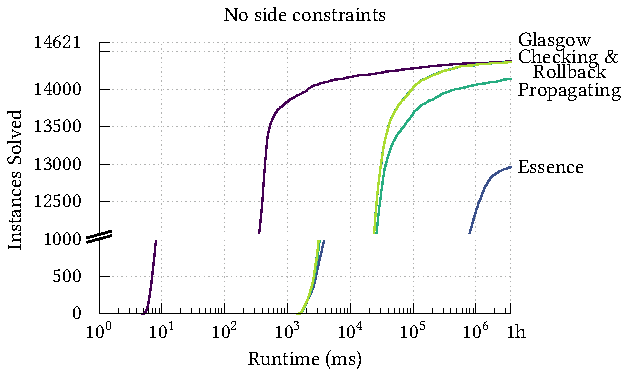
\includegraphics{gen-graph-nosideconstraints.pdf}\hfill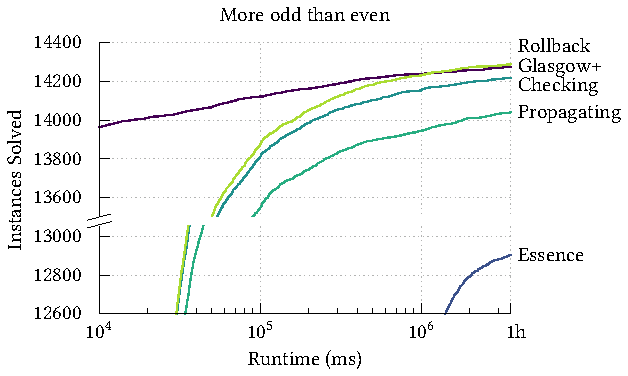
\includegraphics{gen-graph-oddeven.pdf}
    \bigskip
    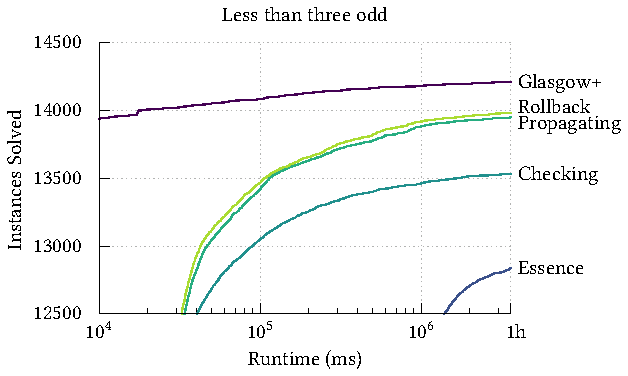
\includegraphics{gen-graph-mostlyodd.pdf}\hfill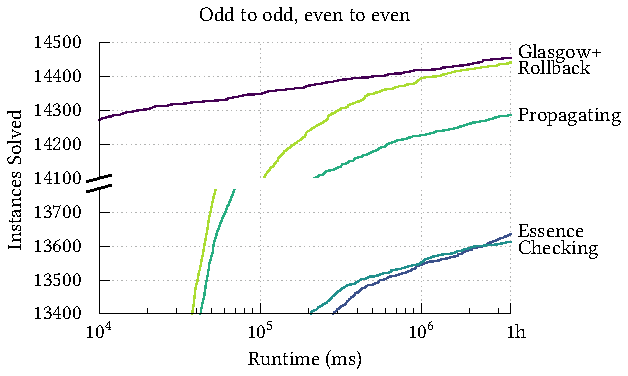
\includegraphics{gen-graph-parity.pdf}
    \caption{Comparing different approaches to hybrid solving. On the top row, ``no side
    constraints'' then with the ``more odd target vertices than even target vertices'' side
    constraint; on the bottom row, the ``mostly odd target vertices'' side constraint on the left,
    and the ``odd to odd, even to even'' side constraint on the right.}\label{figure:cumulative}
\end{figure}

We now present the results of some computational experiments. The experiments in this section are
designed to be hard, and to emphasise the difference between the approaches, rather than to be
realistic. We will continue to work with Solnon's non-induced subgraph isomorphism benchmark
instances, but will consider three variations. Firstly, we will consider the problem with no side
constraints. This is, in some sense, the worst case scenario, where we must pay the full price of
hybrid solving, but cannot get any benefit from it. Secondly, let's say that the number of odd
target vertices used must be greater than the number of even target vertices used:
\newcommand{\modsymbol}{\%}
\begin{lstlisting}
such that (sum i : P . f(i) (*\modsymbol{}*) 2) >
    (sum i : P . (f(i) + 1) (*\modsymbol{}*) 2)
\end{lstlisting}
Thirdly, let us say that fewer than three odd target vertices may be used:
\begin{lstlisting}
such that (sum i : P . f(i) (*\modsymbol{}*) 2) < 3
\end{lstlisting}
And fourthly, let us say that even pattern vertices must be mapped to even target vertices, and odd
pattern vertices to odd target vertices:
\begin{lstlisting}
such that forAll a : P . (a (*\modsymbol{}*) 2) = (f(a) (*\modsymbol{}*) 2)
\end{lstlisting}

We chose these last three problems because intuitively, the first is likely not to be able to
perform inference until deep in a search tree (when most pattern vertices are mapped to specific
target vertices), the second is likely to be able to perform inference early in the search tree
(after a few assignments have been made, but not at the root node), and the third will propagate
only at the root node.

The results of these experiments are presented in
\cref{figure:cumulative}. Let us first look at the top left plot, where we do not actually have any side constraints. When calling
the CP solver as a solution checker, we ultimately achieve the same performance as the Glasgow
Subgraph Solver\footnote{Actually, because high level modelling can use different names for
variables and values, we get slight differences due to changes to tiebreaking in search order
heuristics.}, although we can pay a substantial startup overhead. This should not be surprising:
with no side constraints, the subgraph solver runs as normal, and will perform just one call to the
CP solver on satisfiable instances. The testing and propagating approaches are both over an order of
magnitude slower: calling the CP solver at every search node is clearly very expensive---although if
we do call the CP solver, having it communicate deletions is not much of an additional overhead.
Finally, all approaches substantially outperform using a CP solver on its own without help from the
subgraph solver.

?? Include a version where Minion doesn't actually get the constraints

What about the remaining three plots in \cref{figure:cumulative}, where we do have side constraints (and so can no
longer compare to the subgraph solver on its own)? As we hoped, we see differences between the three
plots. On the top right, where we expect the side constraints to fire late, solution
checking clearly beats testing or propagation during search. However, on the bottom left,
where we expect side constraints to fire early, the testing and propagating approaches are much
better than solution checking. ?? Bottom right. Finally, any approach using the subgraph solver
remains much better than a pure CP approach.

\subsection{A Rollback Approach}

From what we have seen so far, it is obviously important to call the CP solver \emph{some} of the
time during search, but too expensive to call it \emph{all} of the time. We will therefore introduce
a new approach, which we call \emph{rollback}. This approach is inspired by backjumping ??cite, as
well as by the conflict analysis methods used in SAT and SMT solvers ??cite and in lazy clause
generating CP solvers ??cite. The idea is as follows.  Firstly, we call the CP solver with full
propagation at the root node, in case we are dealing with a particularly rich labelling scheme.
Secondly, we use the CP solver for solution checking, since this is required for correctness. Now,
suppose the CP solver rejects a candidate solution: this will cause the subgraph solver to
backtrack. At this point, we call the CP solver again, with full propagation. Either the CP solver
is happy, in which case we proceed with search, or the CP solver indicates failure, in which case we
backtrack again, and do another attempt at full propagation, and so on until the CP solver is happy.

The idea behind this approach is to avoid calling the CP solver when it is unlikely to do anything
useful, but that once a failure has been encountered, we want to extract as much information as we
can from the CP solver. If the failure encountered was due to a ``local'' property of the solution,
such as in the ``more odd than even'' example, then we will quickly return to just using the
subgraph solver for search. However, if the failure is due to only a few early assignments, as in
the ``fewer than three odd vertices'' example, then we will jump back to nearly the root of the
search tree.

The results in \cref{figure:nosideconstraints,figure:oddeventhreeodd} demonstrate the
success of this approach. When there are no side constraints, this approach has no overheads
compared to solution checking. When constraints fire late, this approach is slightly better than
solution checking, and when constraints fire early, this approach is slightly better than always
testing or propagating during search. In other words, rolling back from failures gives us all of the
strengths and none of the weaknesses of the simpler approaches.

?? Randomly also calling in unsat trees?

\section{Subgraph Problems with Side Constraints}

\subsection{Retyping Problems}\label{section:typegraphs}

A \emph{typed graph} is a kind of labelled graph where the labels also carry a graph structure
??cite. In general, mappings between typed graphs must preserve the label structure, but here we
will be looking at a problem variation involving relabelling which occurs in ??application. We may
describe typed graph subisomorphism problems in Essence as follows. As before, we are given a
pattern graph and a target graph, both of which carry labels; we will draw the vertex labels from
different sets, to emphasise
the relabelling.
\begin{lstlisting}
given pl, tl, e : int
letting PL be domain int(1..pl)
letting TL be domain int(1..tl)
letting E be domain int(1..e)
\end{lstlisting}
We are also given labelled graphs,
\begin{lstlisting}
given p, t : int
letting P be domain int(1..p)
letting T be domain int(1..t)

given pat : function (P, P) --> E
given tgt : function (T, T) --> E
given plab : function (total) P --> PL
given tlab : function (total) T --> TL
\end{lstlisting}
but now the labels also carry a graph structure,
\begin{lstlisting}
given pattype : function (PL, PL) --> E
given tgttype : function (TL, TL) --> E
\end{lstlisting}
We are looking for an injective mapping from the pattern graph to the target graph,
\begin{lstlisting}
find f : function
    (total, injective) P --> T
\end{lstlisting}
as well as an injective mapping between the label graphs,
\begin{lstlisting}
find r : function
    (total, injective) PL --> TL
\end{lstlisting}
in such a way that graph structure and labels are preserved,
\begin{lstlisting}
such that forAll (a,b) in defined(pat) .
    pat((a,b)) = tgt((f(a), f(b)))
such that forAll a : P .
    r(plab(a)) = tlab(f(a))
\end{lstlisting}
and also requiring that the structure on the labels is preserved,
\begin{lstlisting}
such that forAll (a,b) in defined(pattype) .
    pattype((a,b)) = tgttype((r(a),r(b)))
\end{lstlisting}

Consider again the example in \cref{figure:littlegraphs}, and now suppose they are equipped with the type
structures shown to the right of each graph,
\begin{lstlisting}
letting pattype be function (
  (1, 1) --> 1, (1, 2) --> 1, (2, 1) --> 1 )
letting tgttype be function (
  (1, 1) --> 1, (1, 2) --> 1,
  (1, 3) --> 1, (3, 1) --> 1 )
\end{lstlisting}
Recall that with vertex relabelling, four solutions exist. However, with retyping, only two of the
solutions respect the type graph,
\begin{lstlisting}
(1 --> 1, 2 --> 3, 3 --> 5)
(1 --> 2, 2 --> 3, 3 --> 5)
\end{lstlisting}
whilst the solutions that instead map pattern vertex 3 to target vertex 4 are no longer valid.

\subsection{Temporal Subgraph Problems}\label{section:temporalgraphs}

In a \emph{temporal graph}, edges are labelled with some kind of timestamp---here we will use
integers. Temporal pattern matching and counting has applications in ??. There are at least three
common kinds of temporal subgraph isomorphism. In an \emph{exact} subisomorphism, times are simply
labels that must match exactly. If we look at \cref{figure:littlegraphs}, now ignoring vertex labels
but using the edge labels,
\begin{lstlisting}
letting l be 1
letting e be 3

letting p be 3
letting pat be function ((1, 2) --> 1, (2, 3) --> 2)
letting plab be function (1 --> 1, 2 --> 1, 3 --> 1)

letting t be 5
letting tgt be function ((1, 3) --> 2, (3, 1) --> 2,
  (2, 3) --> 1, (3, 4) --> 2, (3, 5) --> 3)
letting tlab be function (1 --> 1, 2 --> 1, 3 --> 1,
  4 --> 1, 5 --> 1 )
\end{lstlisting}
then there are two solutions,
\begin{lstlisting}
(1 --> 2, 2 --> 3, 3 --> 1)
(1 --> 2, 2 --> 3, 3 --> 4)
\end{lstlisting}

A less strict kind of subisomorphism is an \emph{offset}, where edge labels must match exactly but
offset by an integer constant. In our example, this means ``find a mapping where the event from 2
to 3 occurs one time unit after the event from 1 and 2''. We can model this as follows:
\begin{lstlisting}
find o : int(-e..e)
such that forAll (a,b) in defined(pat) .
    pat((a,b)) = o + tgt((f(a), f(b)))
\end{lstlisting}
and we find one additional solution,
\begin{lstlisting}
(1 --> 1, 2 --> 3, 3 --> 5)
\end{lstlisting}

Finally, in an \emph{order} embedding, the pattern edge labels simply define an order on events. We
can model this as follows:
\begin{lstlisting}
find o : function (total) E --> E
such that forAll x : int(1..e - 1) .  o(x) <= o(x + 1)
such that forAll (a,b) in defined(pat) .
    pat((a,b)) = o(tgt((f(a), f(b))))
\end{lstlisting}
which gets us yet another solution,
\begin{lstlisting}
(1 --> 2, 2 --> 3, 3 --> 5)
\end{lstlisting}

\subsection{Compiler Instruction Generation}

\subsection{Subgraph Isomorphism With Costs}

We can also support optimisation problems. If, for example, each target vertex has a cost associated with it,
\begin{lstlisting}
given tcost : function (total) T --> int
\end{lstlisting}
then we can ask to find the cheapest solution,
\begin{lstlisting}
minimising sum([ tcost(f(a)) | a : P])
\end{lstlisting}

\section{Conclusion}

\bibliographystyle{splncs04}
\bibliography{paper}

\end{document}

